% catalogue: title = Flowchart with styles and positioning
% catalogue: min-coverage = 0.87
\documentclass[border=10pt]{standalone}
\PassOptionsToPackage{dvipsnames,svgnames,x11names}{xcolor}
\usepackage{tikz}
\usepackage{pgfplots}
\pgfplotsset{compat=newest}
\usepgfplotslibrary{groupplots}
\usetikzlibrary{arrows.meta,positioning,shapes.geometric}
\begin{document}
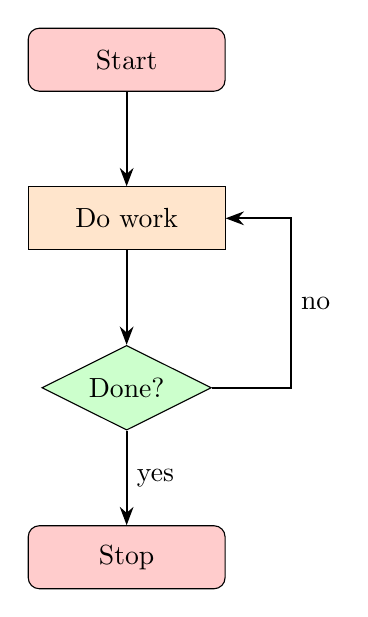
\begin{tikzpicture}[
    node distance=1.2cm,
    startstop/.style={rectangle, rounded corners, minimum width=2.5cm, minimum height=8mm, draw, fill=red!20},
    process/.style={rectangle, minimum width=2.5cm, minimum height=8mm, draw, fill=orange!20},
    decision/.style={diamond, aspect=2, draw, fill=green!20},
    arrow/.style={thick, ->, >=Stealth}
]
    \node[startstop] (start) {Start};
    \node[process, below=of start] (work) {Do work};
    \node[decision, below=of work] (done) {Done?};
    \node[startstop, below=of done] (stop) {Stop};
    \draw[arrow] (start) -- (work);
    \draw[arrow] (work) -- (done);
    \draw[arrow] (done) -- node[right] {yes} (stop);
    \draw[arrow] (done.east) -- ++(1, 0) |- node[near start, right] {no} (work.east);
\end{tikzpicture}
\end{document}
